\documentclass[handout]{beamer}
%
%\mode<presentation>
%{
  \usetheme{Copenhagen} %type de présentation
  %\usecolortheme{blue}% couleur

  %\setbeamercovered{transparent} %laisse le texte à paraître en gris
%}
\usepackage[T1]{fontenc}
\usepackage[utf8]{inputenc}
\usepackage{lmodern}
\usepackage[frenchb]{babel}
\usepackage{amsmath}
\usepackage{amsfonts}
\usepackage{amssymb}
\usepackage{cancel}
\usepackage{mathtools}
\usepackage{array}
\newcommand{\Tau}{\mathrm{T}}


\frenchspacing

\allowdisplaybreaks %?
\let\Tiny=\tiny %pour enlever message erreur: Font shape `OT1/cmss/m/n? in size <4> not available
                %(Font) size <5> substituted on input line...

%\beamerdefaultoverlayspecification{<+->}


%-----------------------------------------------------------------------------------------------------------------
\title{Du Big Bang à l'apocalypse:\\ }
\subtitle{Symétries et solitons dans la cosmologie}
\author{Éric Dupuis}
\institute{Université de Montréal, département de physique \\
Conférences du vendredi des stagiaires}
\date{04-07-2014}


%-----------------------------------------------------------------------------------------------------------------

\begin{document}

%titre
\begin{frame}
\titlepage
\end{frame}
%

\begin{frame}\frametitle{Bonne fête Boson de Higgs!: 4 juillet 2012 - ...}
\begin{figure}
  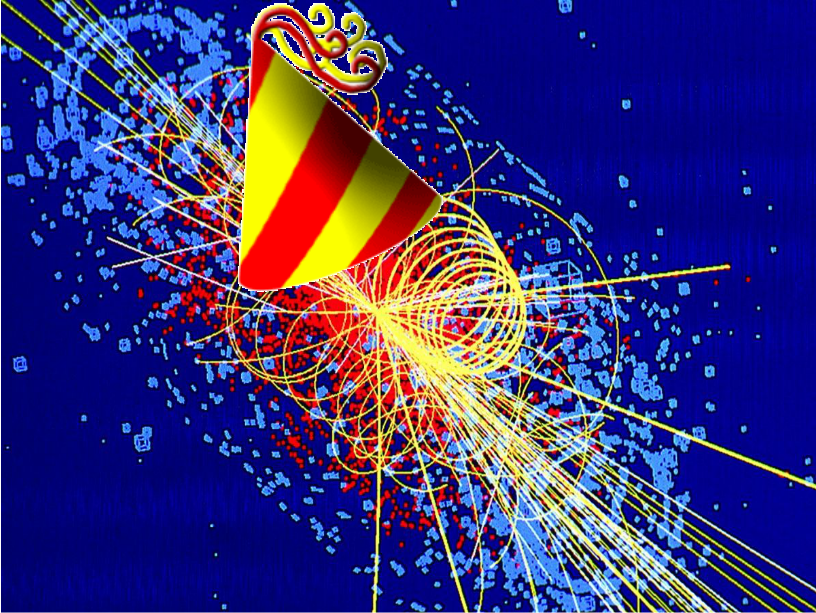
\includegraphics[scale=0.35]{higgsfete.png}
   %+ orientés désorientés ou juste tableau?
 \end{figure}
\end{frame}

\section*{}
\begin{frame}
\tableofcontents
\end{frame}



\section{Cosmologie}
\subsection{Cosmologie 101}
\begin{frame}
\frametitle{Cosmologie 101}
\begin{enumerate}
\item Cosmologie: Structure/origine/évolution de l'univers
\begin{enumerate}
\item Big Bang
\item Modèles inflationnistes
\item Expansion de l'univers
\end{enumerate}
\item Règles et configurations 
\end{enumerate}
 \begin{figure}
  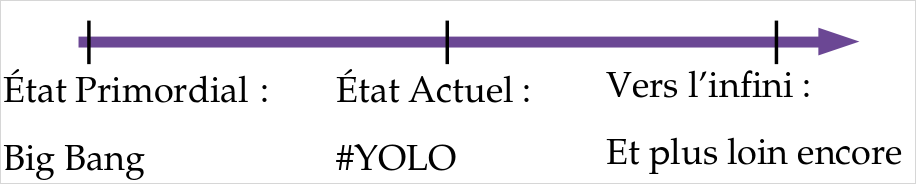
\includegraphics[scale=0.3]{yolo.png}
   %+ orientés désorientés ou juste tableau?
 \end{figure}
\end{frame}


%\begin{frame}
%\begin{block}{Questions fondamentales (style cosmo)}
%\begin{enumerate}
%\item D'où venons-nous? (État primordial de l'univers)
%\item Qui sommes-nous? (État actuel de l'univers)
%\item Où allons-nous? (Évolution de l'univers)
%\end{enumerate}
%\end{block}
%%\begin{figure}[0.5\textwidth]
%%  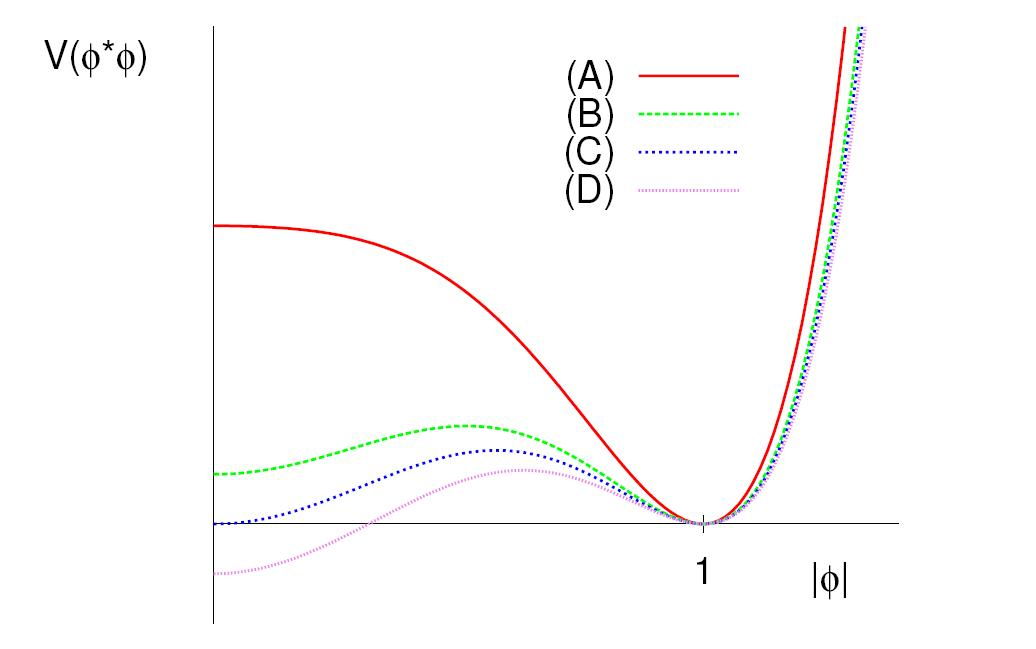
\includegraphics[scale=0.25]{evo_pot.jpg}
%%   %+ orientés désorientés ou juste tableau?
%% \end{figure}
%\end{frame}

\begin{frame}\frametitle{État d'origine $\rightarrow$ État actuel}
\begin{columns}[T]
 \begin{column}[T]{.5\linewidth}
 Big Bang:\\ -Matière compressée\\ -Température très élevée\\ -\textbf{État instable}\\[1 cm]
 \textbf{Forme symétrique:} Importance en cosmologie 
 \end{column}
 \begin{column}[T]{.5\linewidth}
 \begin{figure}[0.5\textwidth]
  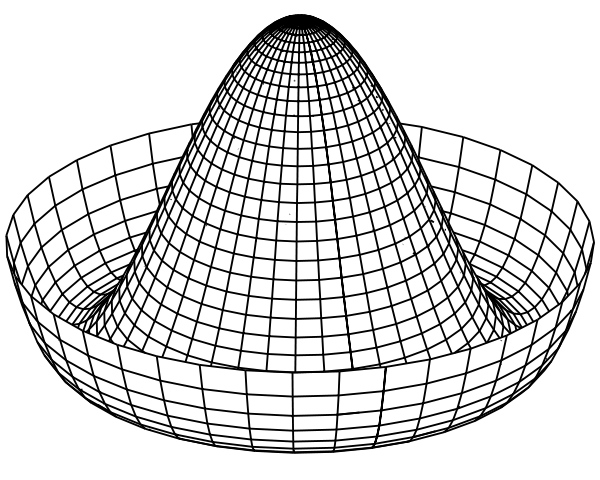
\includegraphics[scale=0.25]{chapeau_mex.png}
   %+ orientés désorientés ou juste tableau?
 \end{figure}
 \end{column}
\end{columns}
\end{frame}


%\item Univers primordial et théorie d'unification (particules)
%\item Atteinte du vide: brisure spontanée de symétrie
%image?



\subsection{Notions de symétrie}
\begin{frame}\frametitle{La symétrie en physique}
\begin{block}{Définition (approximative)}
La \textbf{symétrie} d'un système physique définit une transformation qui le laisse invariant.\\
Théorème de Noether: $\text{Symétries} \leftrightarrow \text{Lois de conservations}$.
\end{block}

%\textsc{Théorème de Nother:} Pour toute transformation infinitésimale laissant l'action invariante, il existe une quantité conservée.

\begin{exampleblock}{Symétrie de l'univers (postultats de la relativité restreinte}
\begin{enumerate}
\item Homogénéitié: Invariance sous translation $\rightarrow$ $\vec{p}$ 
\item Isotropie: Invariance sous rotation $\rightarrow$ $\vec{L}$
\end{enumerate}
\end{exampleblock}
\textbf{Groupe:} Fermeture, Identité, Inverse, Associativité.\\  Symétries $\leftrightarrow$ Générateurs du groupe.\\
Exemple: U(n), O(n), SU(n), SO(n)
\end{frame}

\begin{frame}\frametitle{Ferroaimant de Heisenberg: Dipôles magnétiques en 2D}

\begin{columns}[T]
 \begin{column}[T]{.5\linewidth}
 \begin{equation*}
H= -J\sum_{i}{\sum_{voisins j}{\vec{S}_i\cdot\vec{S}_j}}
\end{equation*} 

\begin{figure}[0.5\textwidth]
   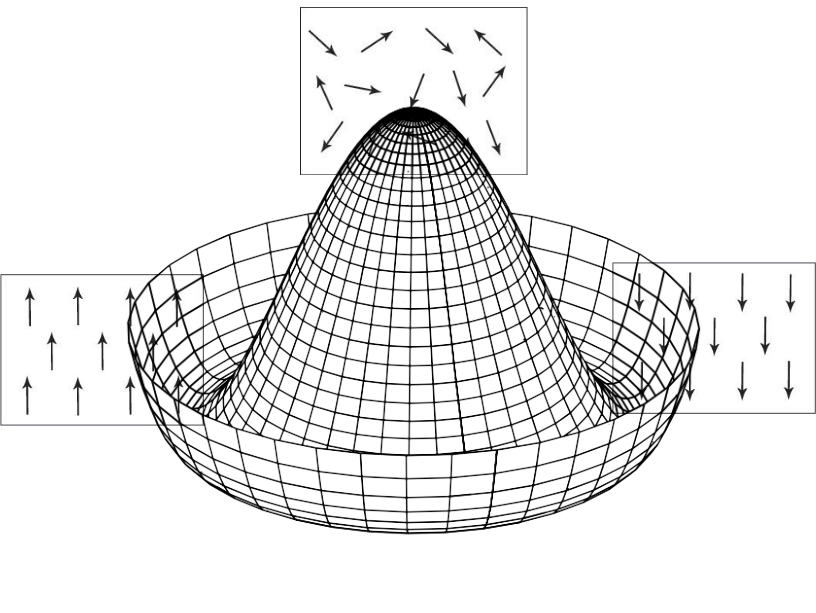
\includegraphics[scale=0.25]{potpot.png}
 \end{figure}
 \end{column}
 \begin{column}{.5\linewidth}

 Invariance de H sous rotation dans le plan \textbf{SO(2)} \\[0.25 cm]
 Vide: Température de Curie
 
  \begin{block}{Brisure spontanée de symétrie}
Les lois de la nature peuvent posséder des symétries qui ne laissent toutefois pas l'état de vide (fondamental) invariant.
\end{block}
  \end{column}
\end{columns}
\end{frame}
%
%\begin{frame}
%    \begin{figure}[0.3\textwidth]
%   %\includegraphics[scale=0.25]{aimants_desorientes.jpg}
%    \end{figure}
%    Petit homme dans le réseau
%    
%Et bien plus encore: vortex pour expliquer les supra type I et II
% \end{frame} 

\begin{frame}\frametitle{Mécanisme de Kibble}


    \begin{figure}[0.3\textwidth]
    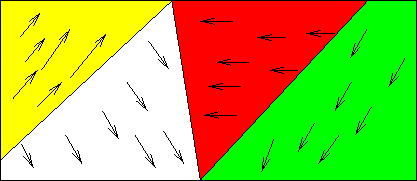
\includegraphics[scale=0.4]{murs.png}
    \end{figure}
Vides dégénérés, différant dans l'espace: défauts topologiques (solitons)


\end{frame}

%
%\begin{frame}\frametitle{Symétries en physique des particules}
%Modèle standard permet les associations suivantes:\\
%\begin{block}{Groupes de Lie, transformations continues}
%\begin{tabular}{ccc}
% Force & Groupe de symétrie & Bosons - Générateurs \\
%  \hline
%  Nucléaire faible & SU(2) & $W^{\pm}$, $Z^0$ \\
%  Nucléaire forte & SU(3)& g \\
%  Électromagnétique & U(1) &  $\gamma$\\
%  &(symétries internes)&
% \end{tabular}
%\end{block}
%\end{frame}


\begin{frame}\frametitle{Brisure de symétrie - Particules}

 \textbf{Grande unification:}
\begin{equation*}
G \rightarrow H \rightarrow ... \rightarrow SU(3) x U(1)
\end{equation*}

\textbf{Symétrie élecrofaible:}  Glashow, Salam et Weinberg
  \begin{equation*}
   SU(2)xU(1)
  \end{equation*}

\textbf{Mécanisme de Higgs:} Bosons de Goldstone \\
\begin{figure}[0.3\textwidth]
    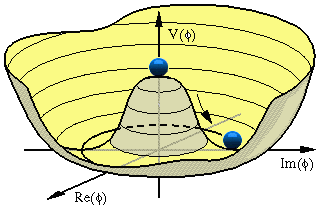
\includegraphics[scale=0.4]{higgs.png}
    \end{figure}


  

\end{frame}



\subsection{Symétrie et cosmologie}
%\begin{frame}
%
%\begin{columns}[T]
%    \begin{column}[T]{.5\linewidth}
%   \begin{figure}[0.3\textwidth]
%    %\includegraphics[scale=0.25]{pot_uni.jpg}
%    \end{figure}
%    \end{column}
%    \begin{column}[T]{.5\linewidth}
%    \begin{enumerate}
%    \item max: univers primordial (densité d'énergie)
%    \item min: notre état de l'univers?
%    \item transition, et apparition d'un vrai vide
%    \begin{enumerate}
%    \item possibilité de transition par effet tunnel
%    \item taux de désintégration; dégéneresence des faux vides
%    \end{enumerate}
%    \end{enumerate}
%        %figure Marie-Lou transition du potentiel
%    \end{column}
%  \end{columns}
%  \end{frame}
  
  \begin{frame}\frametitle{Fin de 1ère section}
  
  
  
\begin{columns}[T]
    \begin{column}[T]{.5\linewidth}
    Supposition: Potentiel V\\[0.5 cm]
    \textbf{1)} Origine $\rightarrow$ max(U), Big Bang\\[0.5 cm]
    \textbf{2)} État actuel 
    \\ $\rightarrow$ symétrie brisée?
    \\ $\rightarrow$ vide métastable? \\[0.5 cm]
	\textbf{3)} Évolution future
	\\ $\rightarrow$ Vers un vrai vide?
	
    \end{column}
    \begin{column}[T]{.5\linewidth}
    \begin{figure}[0.3\textwidth]
    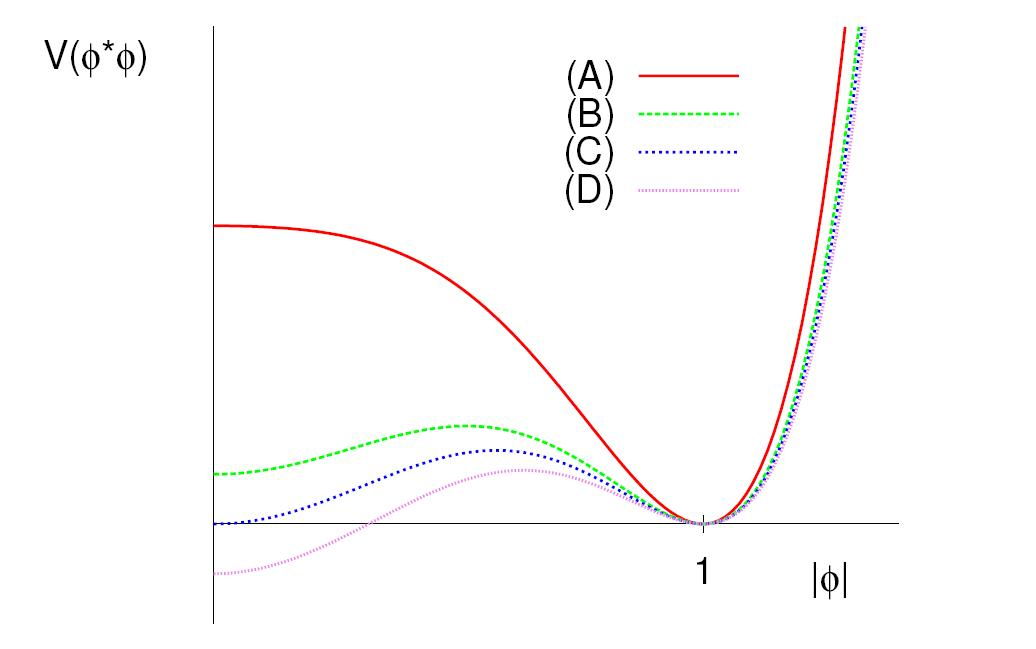
\includegraphics[scale=0.2]{evo_pot.jpg}
    \end{figure}
    
    \end{column}
  \end{columns} 
    \end{frame} 

%    Symétries brisées spontanément: structure non triviale des vides
%    \textbf{Le taux de désintégration de l'univers peut être affecté par la présence de défauts topologiques. Est-ce que l'univers a connu une transition de phase avec brisure de symmétrie? Selon le modèle standard, possiblement. Alors, on attend des cordes cosmiques, monopôles magnétiques. Surtout, ces défauts topologiques pourrait affecter l'évolution actuelle de notre univers. C'est l'objet de notre étude.}
%    



%-----------------------------------------------------------------------------------------------------------------
\section{Solitons - Appareillage mathématique }

\begin{frame}\frametitle{Solitons}
\textbf{Brisure de symétrie:} \\$\rightarrow$
Défauts topologiques: signature des solitons\\
(Ils sont parmi nous?)\\[1 cm]

\textbf{Intérêt cosmologique:} 
%\\$\rightarrow$ Défaut topologique: configurations stables de matières formées lors de la transition de phase 
\\$\rightarrow$ Influence sur le taux de transition vers un vrai vide
      
\end{frame}

\subsection{Équation d'ondes et soliton}
%eq d'onde
\begin{frame}\frametitle{Équation d'ondes et solitons}
Champ scalaire défini dans $\mathbb{R}^d$: $\phi(\vec{x},t)$ (champ???)
\begin{block}{$V=0$}
\textbf{
Équation d'onde:} $\frac{1}{c^2}\frac{\partial^2 \phi}{\partial t^2} - \nabla^2 \phi = \square \phi = 0 $\\[0.25 cm]
\textbf{1)} Forme et vitesse de l'onde conservées
\\\textbf{2)} Deux ondes retrouvent asymptotiquement leur forme/vitesse\\[0.25 cm]
\end{block}



\begin{exampleblock}{$V \neq 0$}

    \textbf{Terme dispersif:} $+m^2\phi$ (Klein-Gordon) 
    \\$\Rightarrow$ $k^2 \rightarrow k^2+m^2$ \\

    \textbf{Terme non-linéaire:} $+\phi^3$\\[0.25 cm]
\begin{columns}[T]
    \begin{column}[T]{.35\linewidth}
    Ondes solitaires \textbf{1)}
    \end{column}
    \begin{column}[T]{.5\linewidth}
    Solitons \textbf{1)}+\textbf{2)} 
    \end{column}
  \end{columns}

\end{exampleblock}




\end{frame}

%%potentiel de solitons
%\begin{frame}
%
%Équation d'onde: V=0
%
%
%\begin{block}{Potentiels différents - Équations du mouvements modifiées}
%\begin{enumerate}
%
%
%\item terme dispersif: $\square\phi +$ \boldmath $m^2 \phi $ \unboldmath  = 0 (Klein-Gordon)\\
%\begin{enumerate}
%\item onde plane: 
%
%\end{enumerate}
%\item terme non-linéaire: $\phi^3$ \\
%\end{enumerate}
%\end{block}
%
%
%\end{frame}

%photo Russell pour le plaisir
\begin{frame}
Sur sa monture, John Russell poursuit sa destinée, vers l'onde solitaire!
\begin{columns}[T]
    \begin{column}[T]{.5\linewidth}
   \begin{figure}[0.3\textwidth]
 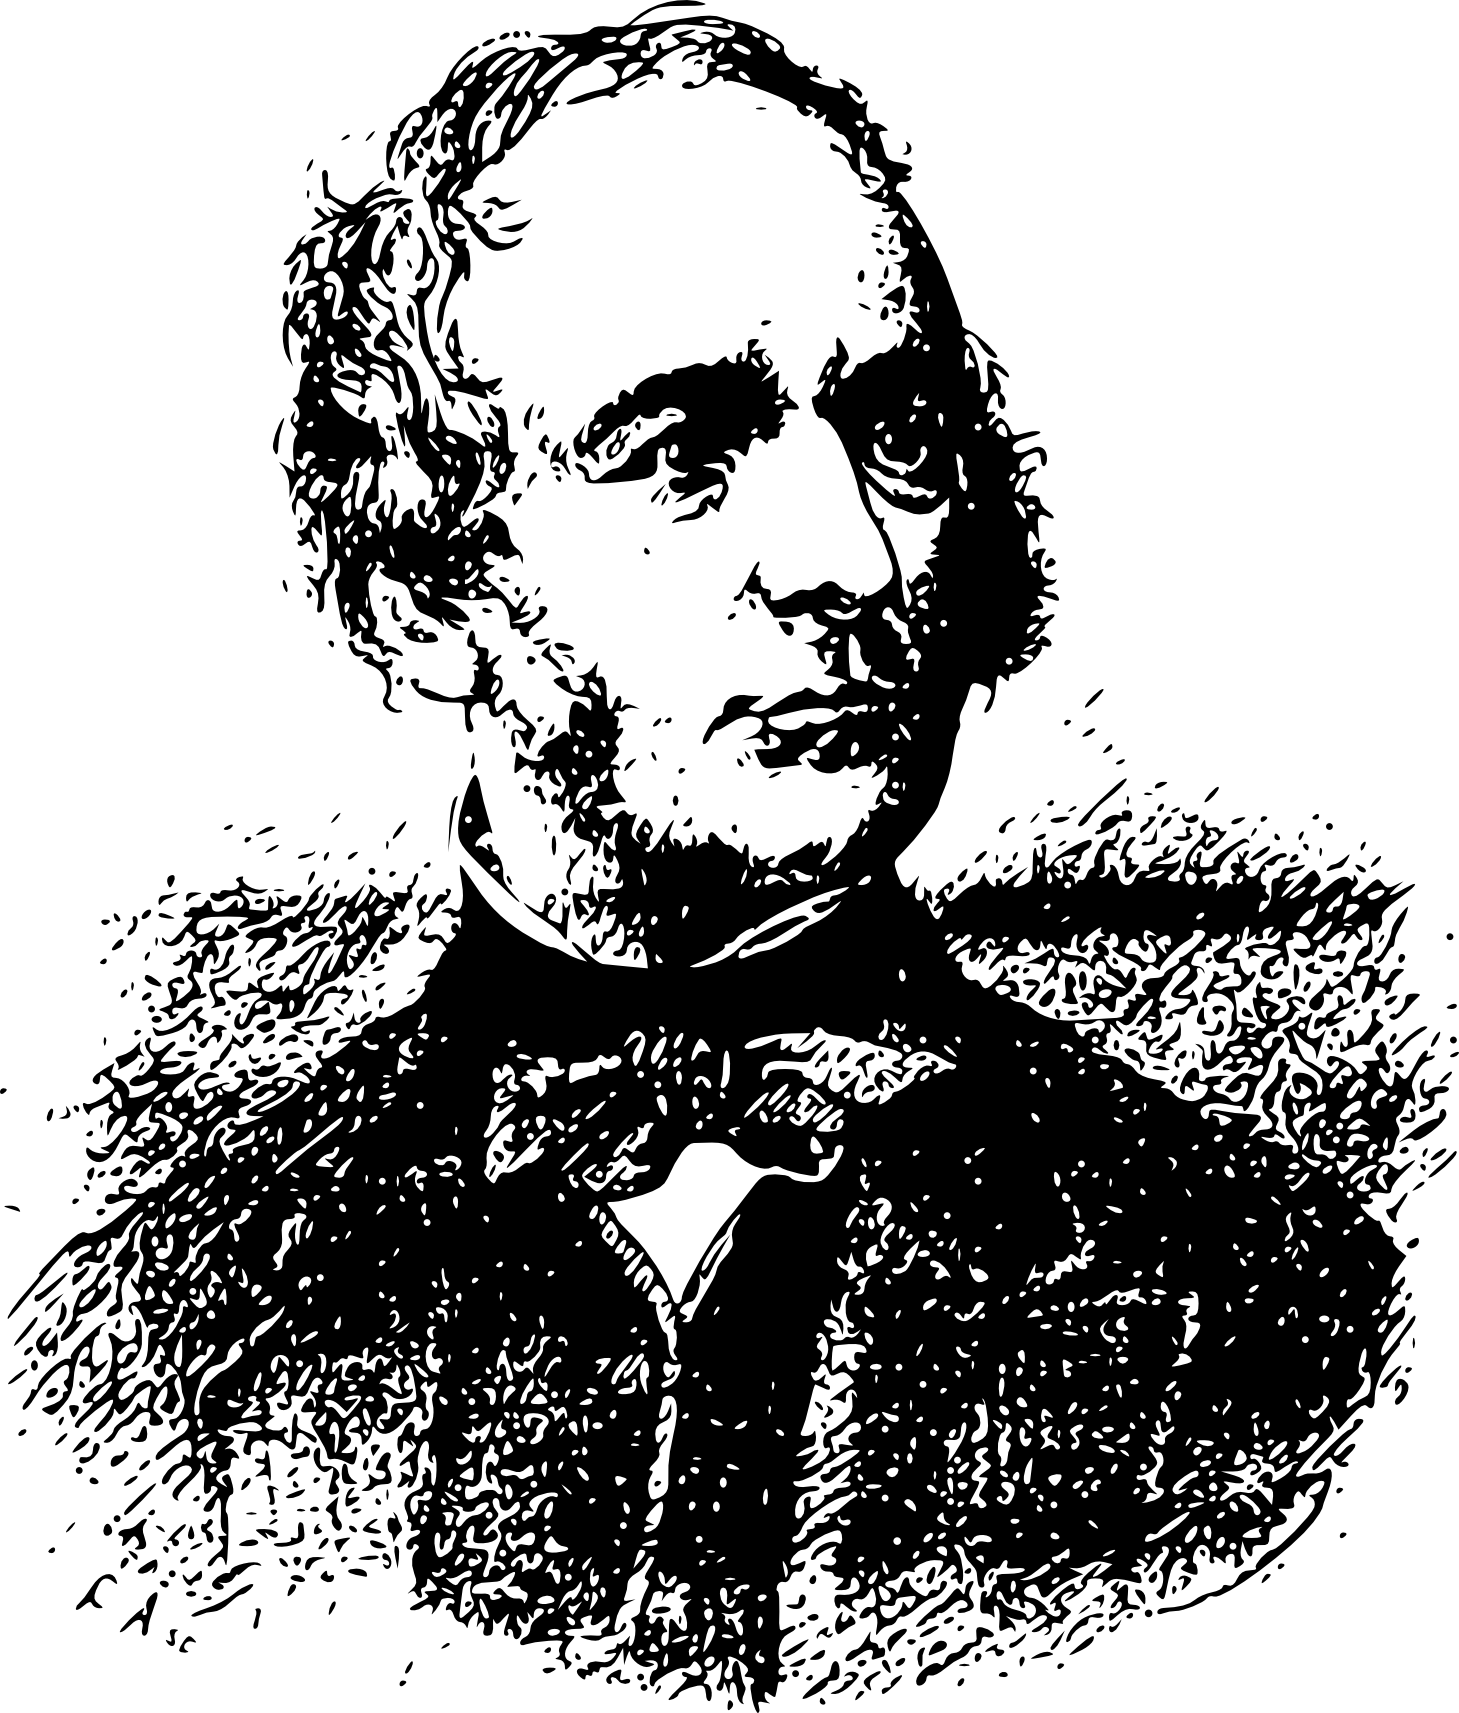
\includegraphics[scale=0.25]{russell.png}
    \end{figure}
    \end{column}
    \begin{column}[T]{.5\linewidth}
    \begin{figure}[0.3\textwidth]
   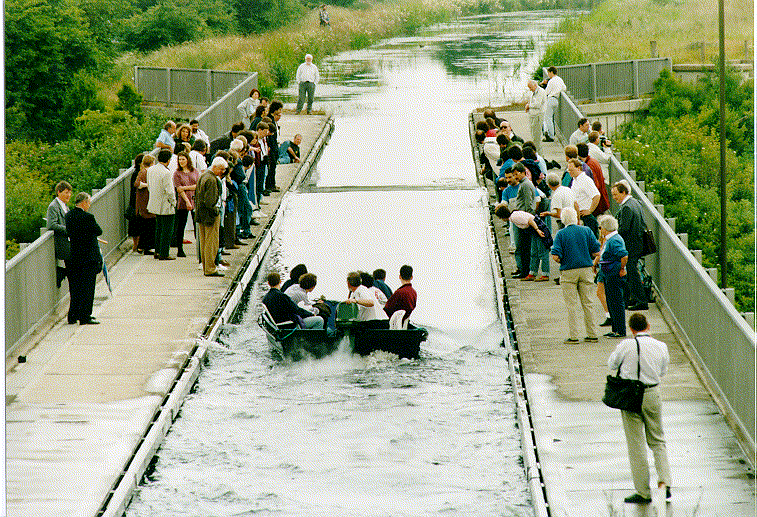
\includegraphics[scale=0.2]{soliton1b.png}
    \end{figure}
    \end{column}
  \end{columns}
\end{frame}

	\begin{frame}\frametitle{En image}

	\begin{figure}[0.3\textwidth]
   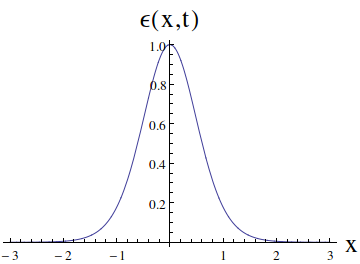
\includegraphics[scale=0.5]{densite.png}
    \end{figure}
    \end{frame}

\begin{frame}\frametitle{Description d'un soliton topologique}

	\textbf{1) Densité d'énergie $\epsilon(x,t)$ d'un soliton (1+1 dim.)} 
	\\$\rightarrow$ Localisée dans l'espace (finitude)
	\\$\rightarrow$ Conservée et non-nulle \\[0.5 cm]

	$\epsilon(x,t) =\mathcal{H}[\phi] = \frac{1}{2} (\partial_x \phi)^2 + V(\phi)$\\[0.25 cm]
%	\begin{align*}
%	E[\phi] = \int{dxdt (\mathcal{H}[\phi])} = \int{dxdt [\frac{1}{2} (\partial_x \phi)^2 + V(\phi)]}
%	\end{align*}
Énergie finie: $\lim\limits_{x \to \pm\infty}\mathcal{H} =0$
	\begin{exampleblock}{}
	$\rightarrow$ $\lim\limits_{x \to \pm\infty}\partial_x \phi =0$
	\\$\rightarrow$  $\lim\limits_{x \to \pm\infty} \phi[x] = g^{(i)}$ où les $g^{(i)}$ sont les min. de V	\\
	\end{exampleblock}
	\textbf{2) Structure des vides non triviale} 
		\end{frame}

	




\subsection{Formalisme Lagrangien}
\begin{frame}

\frametitle{}
\begin{block}{}
Invariant de Lorentz: $x_\mu x^\mu$
\begin{align*}
x^\mu = (x_0,\vec{x}) &\hspace{1 cm} x_\mu = (x_0,-\vec{x})\\
\partial^\mu =& (\frac{1}{c} \partial_t, -\nabla) \\
\partial_\mu \partial^\mu =& \frac{1}{c^2} \partial_t^2- \nabla^2 
\end{align*}

\end{block}
(Indices répétés: Notation d'Einstein)

%\begin{enumerate}
%\item $x_0 = ct \hspace{1 cm} x_{1,2,3} = x,y,z$
%\item Métrique: $x^\mu = g^{\nu\mu} x_\nu$
%\item Minkowski: $\eta^{\nu\mu} \rightarrow diag(1,-1,-1,-1)$
%\end{enumerate}
\end{frame}

\begin{frame}
\begin{enumerate}
\item \textit{Principe d'Hamilton:} $\phi_0$ | action minimisée \\
\item \textit{Action}: $S[\phi] = \int{dt (L[\phi])}  =  \int{d^{\mu}x (\mathcal{L}[\phi])}$\\[0.5 cm]
\item min(S) $\underset{Exp. Taylor}{\implies}$ Premier ordre nul \\
$\Rightarrow$ \textit{Euler-Lagrange:} $\partial_\mu \left(\frac{\partial\mathcal{L}}{\partial(\partial_\mu\phi)}\right) = \frac{\partial\mathcal{L}}{\partial\phi}$\\[0.5 cm]
\item  \textit{Théorie des champs:} $\mathcal{L}[\phi] = \frac{1}{2} \partial_\mu \phi (\partial^\mu \phi)^* -V$

\end{enumerate}
\begin{exampleblock}{Équation d'ondes - V=0}
\begin{align*}
 \partial_\mu(\frac{\partial_a\phi (\partial^a\phi)^* }{\partial_\mu \phi}) = 0 \rightarrow
\partial_\mu (\partial^\mu \phi)^*  = 0 \rightarrow
 \square \phi = 0 \\
\end{align*}
\end{exampleblock}
\end{frame}



\subsection{Kink}
\begin{frame}\frametitle{Kink: cas de figure typique}
\begin{columns}[T]
    \begin{column}[T]{.5\linewidth}
    \begin{exampleblock}{Sous: $\phi \rightarrow -\phi$ $(Z_2)$}
    \begin{align*}
    \mathcal{L} \rightarrow& \mathcal{L}\\
    \phi_0 \rightarrow& -\phi_0 \\
    \end{align*}    
    \end{exampleblock}
%    L'état de vide n'est pas invariant\\[0.5 cm]
    Théorie des champs:
\\$\rightarrow$ Champ scalaire $\phi \hspace{1mm} \epsilon \hspace{1mm} \mathbb{R}$
    \\$\rightarrow$ 1+1 dimensions
  \\$\rightarrow$ solutions statiques \\[0.5 cm]
\end{column}
    \begin{column}[T]{.5\linewidth}
    \begin{block}{}
    \begin{align*}
      V(\phi) = \frac{\lambda}{4}(|\phi|^2 -\frac{m^2}{\lambda})^2
\end{align*}      
      \end{block}
    \begin{figure}
     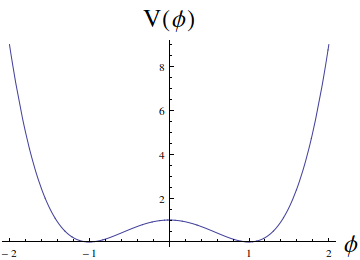
\includegraphics[scale=0.4]{pot_z2.png}
    \end{figure}
    \end{column}
\end{columns}
\end{frame}

\begin{frame} \frametitle{Analogie mécanique classique}
\begin{equation*}
\mathcal{H}[\phi] = \frac{1}{2} \partial_\mu \phi (\partial_\mu \phi)^* +V
\end{equation*}
\begin{columns}[T]
    \begin{column}[T]{.55\linewidth}
    Champ
    \begin{enumerate}
    \item $\mathcal{H} =  \cancelto{}{\frac{1}{2}  (\partial_t \phi)^2} +  \frac{1}{2}  (\partial_x \phi)^2 +V(\phi) $
%    \item $\frac{\partial^2\phi}{\partial_x^2} = \frac{\partial V}{\partial\phi}$
    \item $E_\phi = \int{dx\left[\frac{1}{2}  (\partial_x \phi)^2 +V(\phi) \right]}$
    \end{enumerate}
    \end{column}
    \begin{column}[T]{.45\linewidth}
	Particule
    \begin{enumerate}
    \item $L =   \frac{1}{2}  \dot{q}^2 -U(q)$
%    \item $\frac{\partial^2\phi}{\partial_x^2} = -\frac{\partial U}{\partial\phi}$
    \item $S_q = \int{dt[\frac{1}{2}  \dot{q}^2 -U(q)] }$
    \end{enumerate}
    \end{column}
  \end{columns}
  \begin{figure}
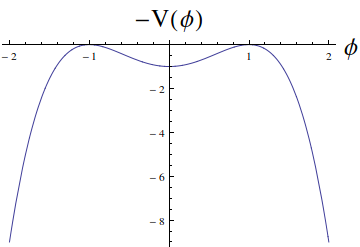
\includegraphics[scale=0.5]{pot_inv.png}
\end{figure}
% 
%    $E_\phi$ finie $\leftrightarrow S_q$ finie $\rightarrow E_q = 0$\\
% On étudie alors: -V

  
\end{frame}

%\begin{frame}
%Récapitulons:
%\begin{enumerate}
%\item 1+1 dimensions, mais solution statique
%\item Potentiel V d'ordre 4 
%\item Équations d'Euler-Lagrange $\rightarrow$ Équations du mouvement: 
%\begin{enumerate}
%
%\item solution: kink
%\end{enumerate}
%\end{enumerate}
%\end{frame}

\begin{frame}\frametitle{Kink}
\begin{columns}[T]

 \begin{column}[T]{.6\linewidth}
 \begin{block}{}
 éq. du mouv.: non-linéaire + dispersif\\
  $\underset{Euler-Lagrange}{\implies} \phi'' = \lambda \phi^3 - m^2 \phi$
\begin{align*}
\phi(x) = \frac{m}{\sqrt{\lambda}}tanh\left[\frac{m}{\sqrt{2}}(x-x_0)\right] \\
\end{align*}
 \end{block}
 
 \begin{exampleblock}{}
   
%  $\underset{E-L}{\implies} \frac{1}{2} \phi'^2 = U(\phi)$ dans $ \mathcal{H}(\phi)=\epsilon(x)$
\begin{align*}
\epsilon(x)= \frac{m^4}{\sqrt{2\lambda}}sech^4\left[\frac{m}{\sqrt{2}}(x-x_0)\right]
\end{align*}
 \end{exampleblock}

 \end{column}
 \begin{column}[T]{.4\linewidth}
\begin{figure}
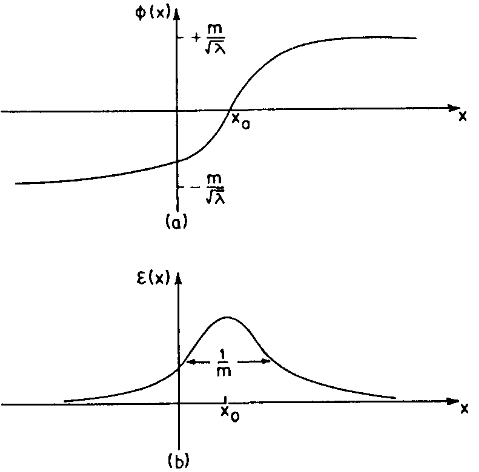
\includegraphics[scale=0.3]{kink_energie.png}
\end{figure}
 \end{column}
\end{columns}
  \end{frame}

\begin{frame}

\begin{figure}
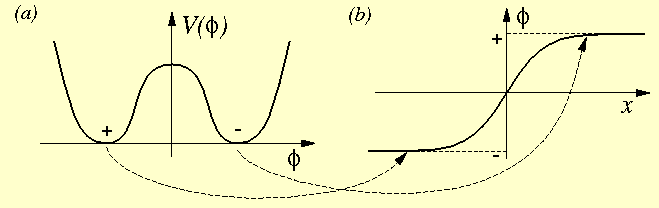
\includegraphics[scale=0.4]{soli_def.png}
\end{figure}
$\phi(x=\infty)- \phi(x=-\infty)$ conservé (charge topologique Q= $\int{k_0 dx}$)
\\$\rightarrow$ Déformations continues impossibles
\\$\rightarrow$ Secteurs topologiques non connectés\\[0.5 cm]

\textbf{Configuration non triviale de vides $\rightarrow$ Solution non dissipative}\\
(Continuité de la solution en x)

%\begin{align*}
%\forall \hspace{1 mm} t \hspace{1 mm} \exists \hspace{1 mm} x \hspace{1 mm} | \hspace{1 mm} \epsilon(x,t) \geq U(\phi=0)\\
%\rightarrow max|_x \epsilon(x,t) > 0
%\end{align*}

%Mur de domaine (symétrie discrète brisée, 1 dimension) \\$\rightarrow$ Cordes cosmiques (cylindrique), monopôles (sphérique)

\end{frame}

\begin{frame}\frametitle{Retour - Cosmologie et solitons}
\begin{enumerate}
\item Symétries brisées dans la nature (\textbf{MS}, ferroaimant)
\end{enumerate}
\begin{enumerate}
\item Structure non triviale des vides dans l'univers\\
$\rightarrow$ défauts topologiques $\rightarrow$ solitons
\item $\Rightarrow$ Mur de domaine (sym. discrète 1 dim.)\\$\Rightarrow$ Corde Cosmique (cylindrique)\\$\Rightarrow$ Monopôle (sphérique)
\item Évolution de l'univers?
\end{enumerate}



\end{frame}

\begin{frame}\frametitle{Taux de désintégration du faux vide}
\begin{columns}[T]
    \begin{column}[T]{.55\linewidth}
   \textbf{Effet tunnel quantique}
        \begin{figure}[.45\linewidth]
    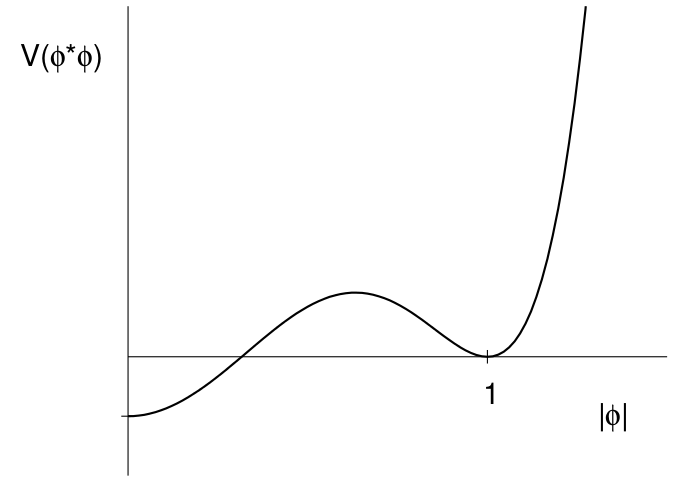
\includegraphics[scale=0.2]{false1.png}
    \end{figure}
 
   % Fluctuations:\\ Quantiques $\leftrightarrow$ Thermodynamiques \\ (Bulles de vrai vide)
    \end{column}
    \begin{column}[T]{.45\linewidth}
   \textbf{Espace Euclidien:} $t\rightarrow i\tau$ \\
    Quantique Min. $\rightarrow$ Classique Euc.
       \begin{figure}
    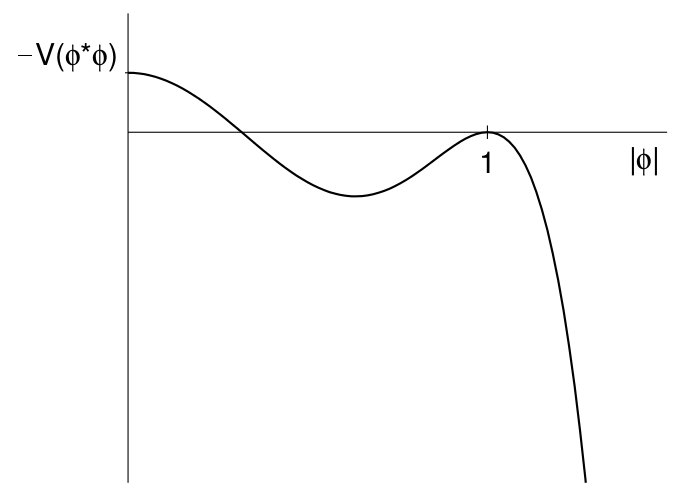
\includegraphics[scale=0.15]{false2.png}
    \end{figure}
 $\rightarrow$ min($S_E$) $\rightarrow$ Bounce, Instanton
 \\$\rightarrow$ Intégrale de chemin: $ \Tau/V \approx e^{-So/\hbar}$    
    \end{column}
\end{columns}
\end{frame}


\begin{frame}
Fluctuation d'un soliton: autre source de désintégration!!!\\
\end{frame}



%-----------------------------------------------------------------------------------------------------------------

\section{Quotidien en cosmologie théorique des particules}
\begin{frame}
%potentiel avec lequel on travaille
\begin{block}{Potentiel à deux champs $\phi(x,t)$ et $\psi(x,t)$}
\begin{equation*}
V(\phi,\psi)=(\psi^2-\delta_1)(\psi^2-1)^2+\frac{\alpha}{\psi^2+\gamma}[(\phi^2-1)^2 - \frac{\delta_2}{4}(\phi-2)(\phi+1)^2] 
\end{equation*}

\end{block}
\begin{columns}[T]
    \begin{column}[T]{.5\linewidth}
  
\begin{enumerate}
\item 1+1 dimensions, on cherche une solution statique
\item Paramètres: $\alpha, \gamma, \delta_1, \delta_2$
\item $\gamma$: couplage
\item $\alpha$: Importance du 2ème terme 
\end{enumerate}  
    \end{column}
    \begin{column}[T]{.5\linewidth}
    \begin{figure}[0.3\textwidth]
    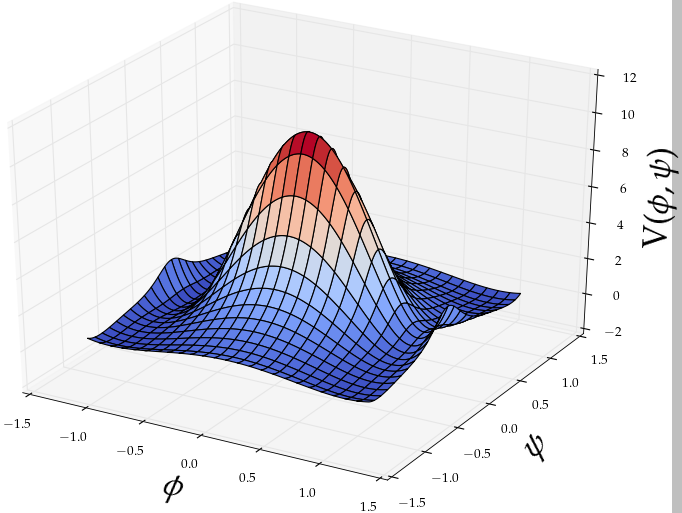
\includegraphics[scale=0.2]{potypot.png}
    \end{figure}
    \end{column}
  \end{columns}
\end{frame}

\begin{frame}
%Pourquoi bâtir un potentiel comme ça en premier lieu?!?!\\  

\begin{figure}[0.3\textwidth]
    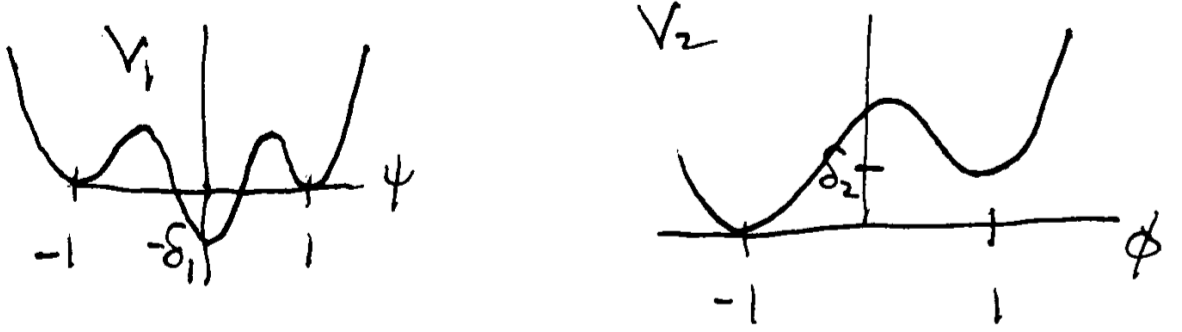
\includegraphics[scale=0.25]{psi_phi.png}
    \end{figure}
\begin{columns}[T]
    \begin{column}[T]{.5\linewidth}
    \begin{enumerate}
    \item $\delta_1 \rightarrow$ contrôle du minimum central
    \item Ordre 6, CLASSIQUE! 
    \end{enumerate}
   
    \end{column}
    \begin{column}[T]{.5\linewidth}
    \begin{enumerate}
    \item $\delta_2 \rightarrow$ Contrôle de la séparation entre minimum sur l'axe $\phi$
    \end{enumerate}

    \end{column}
  \end{columns}

\end{frame}

\begin{frame}\frametitle{À venir...}
Solutions aux équations de mouvements (contraintes à $\lim\limits_{x \to \pm\infty}$)

  \begin{figure}
     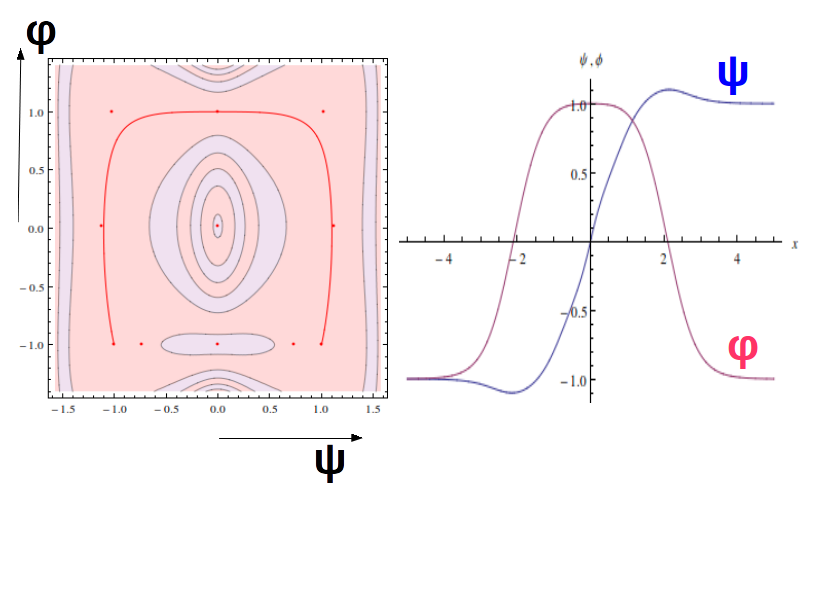
\includegraphics[scale=0.35]{collageener.png}
    \end{figure}
%
%\begin{columns}[T]
%    \begin{column}[T]{.5\linewidth}
%    \begin{figure}
%    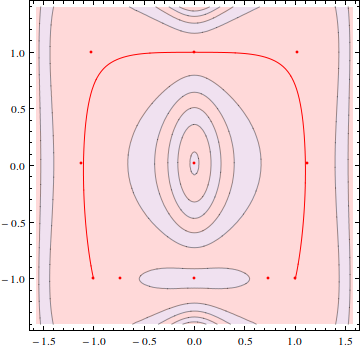
\includegraphics[scale=0.35]{traj.png}
%    \end{figure}
%    \end{column}
%
%    \begin{column}[T]{.5\linewidth}
%    \begin{figure}
%    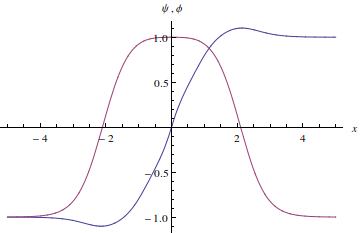
\includegraphics[scale=0.45]{phi_psi.png}
%    \end{figure}
%    \end{column}
%\end{columns}
    
\end{frame}

\begin{frame}
Tester la stabilité de la solution\\[0.5 cm]
 Trouver une borne maximale sur l'action $\rightarrow$ borne minimale sur $\Tau$

  \begin{figure}
     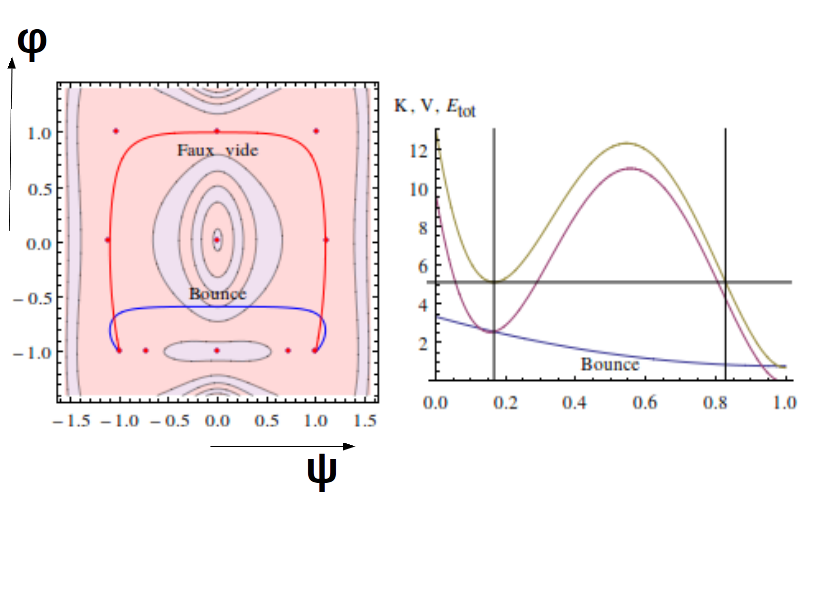
\includegraphics[scale=0.35]{ener2.png}
    \end{figure}
%    \begin{columns}[T]
%        \begin{column}[T]{.5\linewidth}
%        \begin{figure}[0.3\textwidth]
%     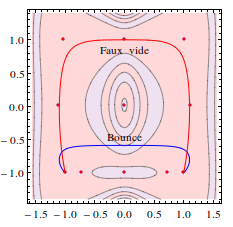
\includegraphics[scale=0.5]{bouncy.png}
%    \end{figure}
%        \end{column}
%    
%        \begin{column}[T]{.5\linewidth}
%        \begin{figure}[0.3\textwidth]
%     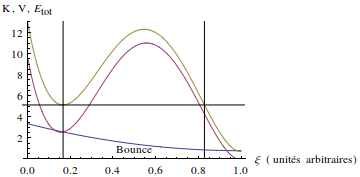
\includegraphics[scale=0.5]{ener.png}
%    \end{figure}
%        \end{column}
%    \end{columns}

    

 
\end{frame}



\end{document}